\section{Experiments: reading the results without overclaiming}
\label{sec:experiments}

\subsection{Three empirical questions}

The paper evaluates D-Tracker with three questions:
\begin{description}[leftmargin=1.8em,style=nextline]
  \item[Q1 --- Accuracy.] How accurately does it forecast compared with strong methods?
  \item[Q2 --- Scalability.] How does runtime change as the stream grows?
  \item[Q3 --- Effectiveness.] Does it extract trend, seasonality, and diffusion in a readable way?
\end{description}
Do not merge these questions. A model can win MAE without explaining diffusion; a beautiful diffusion
map does not prove good forecasting. Read the section as three separate views of one model.

\subsection{Data}

The paper uses five GoogleTrends streams and one COVID-19 stream. Table~\ref{tab:datasets} is copied
from paper Table~4; shapes are ordered (time, keywords, locations).

\begin{table}[htbp]
  \centering
  \small
  \caption{The six datasets in the paper (paper Table~4). Keyword names are preserved.}
  \label{tab:datasets}
  \begin{tabular}{@{}cl>{\raggedright\arraybackslash}p{5.6cm}c@{}}
    \toprule
    ID & Dataset & Keywords & Shape \\
    \midrule
    1 & Device & Apple Watch, Fitbit, Galaxy, Google Pixel, Macbook, Xperia, iPad, iPhone & $(676,8,50)$ \\
    2 & Pythonlib & matplotlib, numpy, pandas, pytorch, scipy, sklearn, tensorflow & $(676,7,50)$ \\
    3 & VoD & Apple TV, DAZN, HBO, Prime Video, hulu, netflix, youtube & $(676,7,50)$ \\
    4 & Chatapp & facebook, instagram, slack, snapchat, tiktok, twitter, viber, whatsapp & $(676,8,50)$ \\
    5 & Language & CSS, HTML, Java, JavaScript, PHP, Ruby, SQL, python, swift & $(676,9,50)$ \\
    6 & Covid-19 & new infected, new deceased & $(990,2,50)$ \\
    \bottomrule
  \end{tabular}
\end{table}

GoogleTrends is weekly data from 2010 to 2022. Covid-19 is daily data from January 2020 to September
2022. Everything is min--max normalized to $[0,1]$. There is a small inconsistency in the paper: the
prose says 48 countries, while paper Table~4 uses 50 locations. This guide preserves both and does not
``fix'' either number.

\subsection{Forecast setup}

For GoogleTrends, the current window is $L_c=104$ weeks (two years), and the horizon is
$L_f\in\{13,26,39\}$ weeks (3, 6, 9 months). For Covid-19, $L_c=56$ days (eight weeks), and
$L_f\in\{7,14,21\}$ days, described as 1, 2, 3 weeks in the results. Baselines are DISMO, FluxCube,
PatchTST, Autoformer, DeepAR, LaST, and CoST. Training and tuning details are in Appendix~B.1; D-Tracker
updates a fixed-window model instead of retraining from the entire history at every step.

\subsection{MAE and RMSE: get the direction right}

For $n$ forecasts, let $y_i$ be the truth and $\hat y_i$ the prediction:
\[
  \mathrm{MAE}=\frac1n\sum_{i=1}^n|y_i-\hat y_i|,
  \qquad
  \mathrm{RMSE}=\sqrt{\frac1n\sum_{i=1}^n(y_i-\hat y_i)^2}.
\]
Both are \textbf{better when smaller}. MAE measures average error; RMSE punishes large errors more
strongly. An illustrative pair of errors $-0.04$ and $+0.08$ gives MAE $=0.06$ and
RMSE $=\sqrt{(0.0016+0.0064)/2}\approx0.063$. This is a made-up metric example, not a paper result.

\begin{commonmistake}
Do not compare a paper Table~3 MAE of $0.84$ directly with an unnormalized raw value of $0.84$. The table
header specifies units of $\times10^{-2}$; this guide preserves the printed values and does not convert
them silently. State the unit whenever you quote them.
\end{commonmistake}

\subsection{Q1: accuracy}

Table~\ref{tab:dtracker-mae} copies only D-Tracker rows from paper Table~3, not baselines. The paper
concludes that D-Tracker has the best MAE on \emph{all} datasets and greatly reduces RMSE, while also
acknowledging that some RMSE values are comparable because RMSE is sensitive to large errors. Both
statements belong together.

\begin{table}[htbp]
  \centering
  \scriptsize
  \caption{D-Tracker MAE and RMSE values from paper Table~3, exactly as printed (table units:
  $\times10^{-2}$). Columns 1/2/3 are the three $L_f$ horizons in the dataset name.}
  \label{tab:dtracker-mae}
  \begin{tabular}{@{}lccccccc@{}}
    \toprule
    & & \multicolumn{3}{c}{MAE} & \multicolumn{3}{c}{RMSE} \\
    \cmidrule(lr){3-5}\cmidrule(lr){6-8}
    Dataset & $L_f$ & 1 & 2 & 3 & 1 & 2 & 3 \\
    \midrule
    Device & 13/26/39 & 0.84 & 0.90 & 0.97 & 1.82 & 1.95 & 2.18 \\
    Pythonlib & 13/26/39 & 0.27 & 0.32 & 0.37 & 1.42 & 1.54 & 1.78 \\
    VoD & 13/26/39 & 0.53 & 0.59 & 0.63 & 1.58 & 1.83 & 2.02 \\
    Chatapp & 13/26/39 & 0.28 & 0.34 & 0.41 & 0.83 & 1.01 & 1.24 \\
    Language & 13/26/39 & 0.31 & 0.35 & 0.40 & 0.97 & 1.14 & 1.32 \\
    Covid-19 & 7/14/21 & 0.47 & 0.70 & 0.98 & 1.40 & 2.42 & 3.65 \\
    \bottomrule
  \end{tabular}
\end{table}

Two headline numbers appear in the final bullet of §1: ``up to 57\% improvement'' and ``up to
8.0$\times$ faster''. The paper does
not state the denominator of 57\% in that sentence, so this guide writes ``the paper reports up to
57\%'', without recomputing it or assigning it to a metric. Likewise, 8.0$\times$ is a result on the
paper's hardware, not a universal constant.

\subsection{Ablation: which component contributes?}

\begin{figure}[htbp]
  \centering
  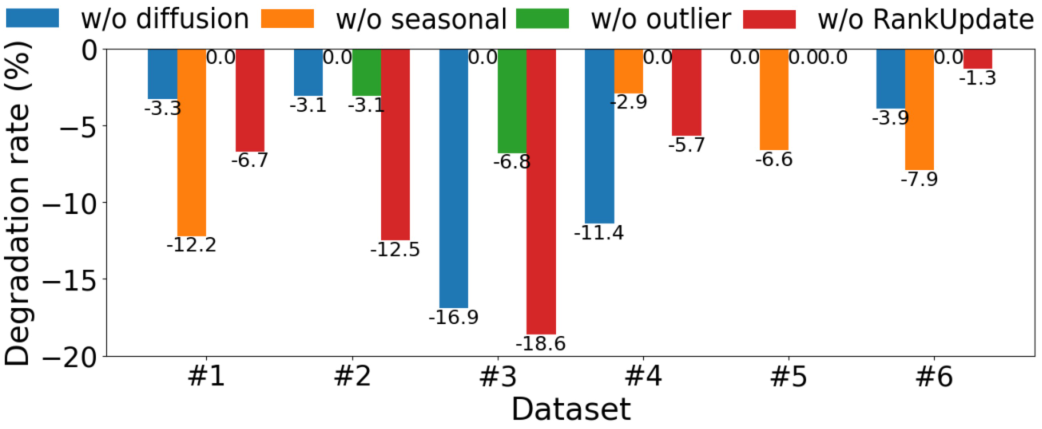
\includegraphics[width=0.95\linewidth]{figures/drop_rate.png}
  \caption{Ablation study. Higher bars represent larger degradation when a component is removed.
  Source: Higashiguchi et al. (2025), arXiv:2505.00242v1, Figure~3; author-owned figure, CC BY 4.0.}
  \label{fig:ablation}
\end{figure}

Figure~\ref{fig:ablation} removes diffusion, seasonal, outlier, and RankUpdate in turn. Degradation
rates are measured at a horizon of 26 weeks (GoogleTrends) or 14 days (Covid-19). The paper reports:
\begin{itemize}
  \item seasonal terms improve datasets with strong seasonality such as Device, Language, and Covid-19;
  \item diffusion improves VoD and Chatapp noticeably;
  \item outliers help some datasets by filtering abrupt changes;
  \item RankUpdate helps the model adapt when the optimal dimension changes.
\end{itemize}
The exceptions matter too. In Language, diffusion does not improve accuracy; the paper suggests there
may be little cross-country diffusion for programming languages. In datasets with few seasonal patterns
or outliers, those components may not help. A model that wins on average does not imply every module
is useful everywhere.

\subsection{Q2: scalability}

\begin{figure}[htbp]
  \centering
  \begin{subfigure}[t]{0.49\linewidth}
    \centering
    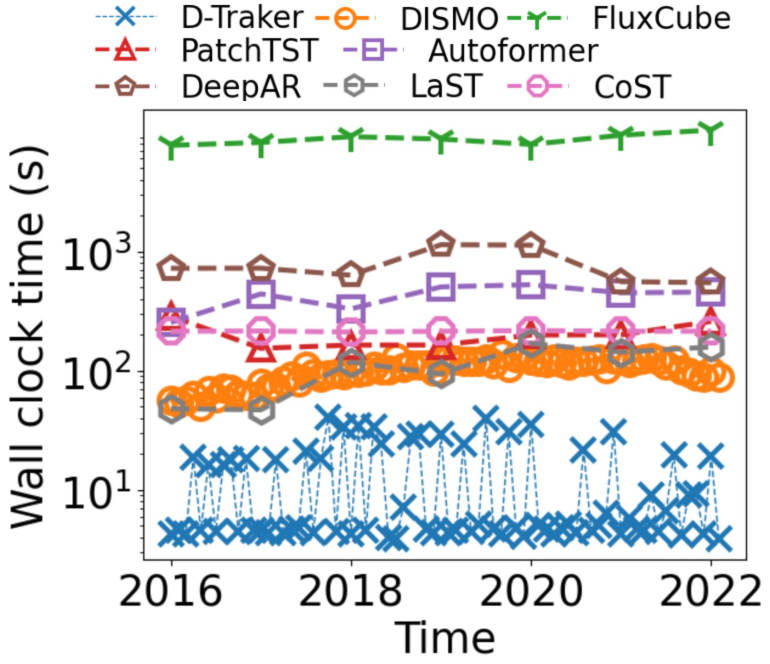
\includegraphics[width=\linewidth]{figures/scalability.png}
    \caption{Time versus stream length.}
  \end{subfigure}\hfill
  \begin{subfigure}[t]{0.49\linewidth}
    \centering
    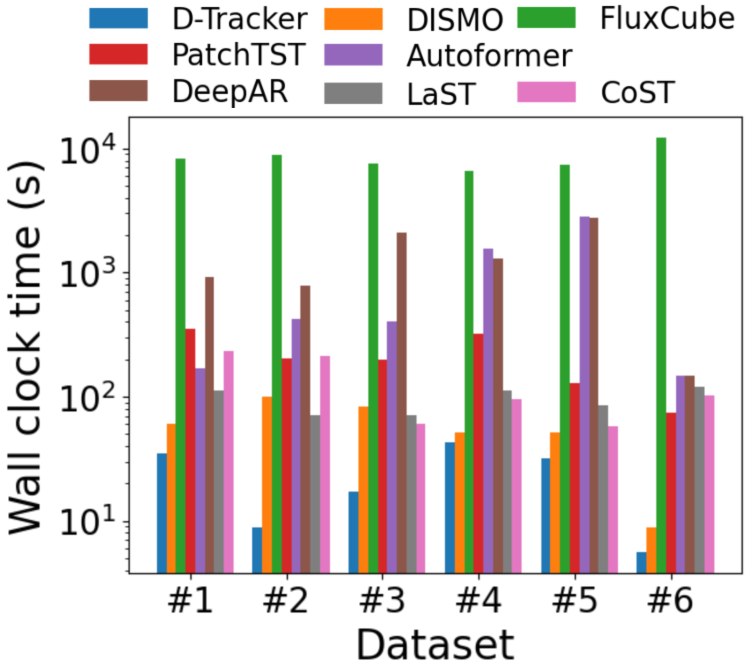
\includegraphics[width=\linewidth]{figures/avgtime.png}
    \caption{Average time over the streams.}
  \end{subfigure}
  \caption{D-Tracker scalability on Pythonlib. Source: Higashiguchi et al. (2025),
  arXiv:2505.00242v1, Figure~4; author-owned figure, CC BY 4.0.}
  \label{fig:scalability}
\end{figure}

In Figure~\ref{fig:scalability}, D-Tracker's processing time is nearly flat as the stream grows, while
baselines tend to rise. The small spikes occur when RankUpdate calls ModelEstimation several times.
This supports the ``time independent of stream length'' claim, but it is not a claim that every
operation is constant: cost still depends on keywords, locations, rank, and structure updates.

\subsection{Q3: is the model interpretable?}

\begin{figure}[htbp]
  \centering
  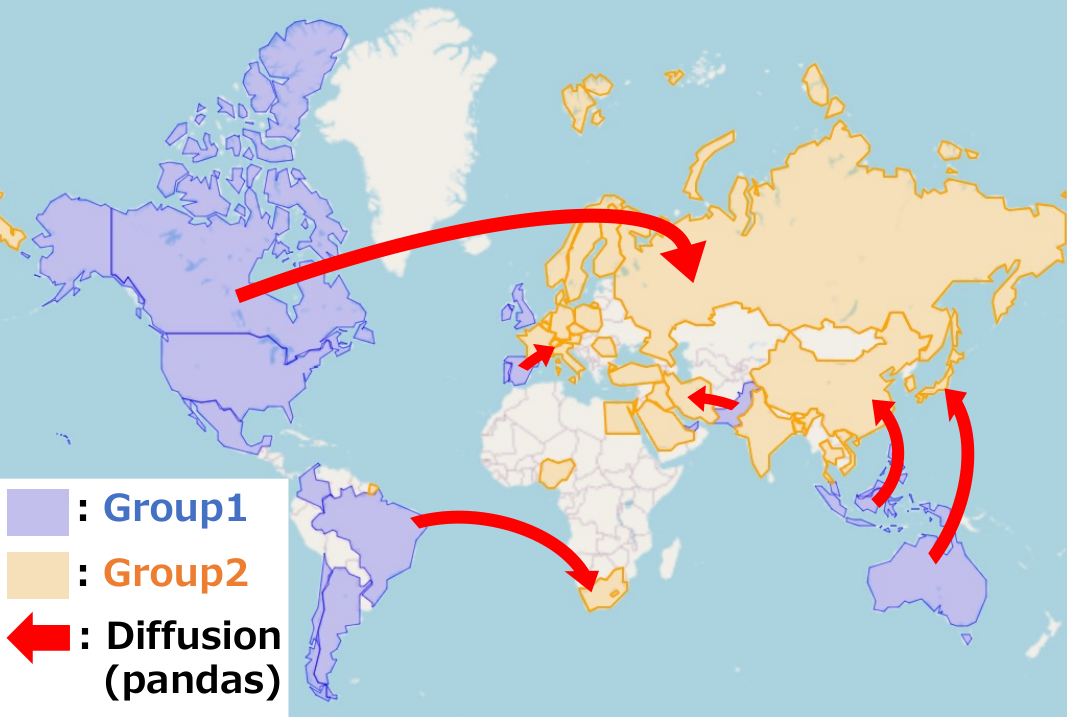
\includegraphics[width=0.78\linewidth]{figures/diff_2014.png}
  \caption{Part of the Pythonlib modeling result for 2013--2015: the reaction--diffusion system's
  diffusion pattern associated with ``pandas''. Source: Higashiguchi et al. (2025),
  arXiv:2505.00242v1, Figure~5; author-owned figure, CC BY 4.0.}
  \label{fig:diffusion-example}
\end{figure}

The paper reads Figure~\ref{fig:diffusion-example} as follows: the dynamics related to ``pandas''
spreads from a location group containing North America and Australia to a group containing Asian
countries, mainly China. This is a \emph{structured interpretation}: the keyword factor says
``pandas'', the location factor defines groups, and diffusion parameters give a direction. It is not
proof of causation; validation requires external evidence or an appropriate experimental design.

\subsection{What the paper does not establish}

The paper reports no confidence intervals, statistical significance tests, or predictive
probabilities. It also does not prove that D-Tracker always beats every baseline at every horizon; the
conclusion is bounded to six streams and the stated settings. The correct sentence is ``in these
experiments, D-Tracker achieved the best MAE and lower runtime'', not ``D-Tracker is the best method
for every time series''.

\begin{keypoint}
Remember three results: (1) D-Tracker leads MAE on all six datasets in paper Table~3; (2) per-step time does
not grow with stream length because of the fixed window, with spikes during rank changes; (3) the model
produces readable groups and diffusion directions, but these are interpretations under assumptions,
not proven causal effects.
\end{keypoint}

\begin{selfcheck}
\begin{enumerate}
  \item Why can MAE and RMSE rank two models differently?
  \item In the ablation, why might removing diffusion fail to hurt Language?
  \item Why does ``time independent of stream length'' not mean $O(1)$?
  \item State one conclusion that \emph{cannot} be drawn from Figure~\ref{fig:diffusion-example}.
\end{enumerate}
\end{selfcheck}
